\documentclass[10pt]{beamer}

% Packages
\usepackage[utf8]{inputenc}
\usepackage[T1]{fontenc}
\usepackage{amsmath, amssymb, amsthm}
\usepackage{graphicx}
\usepackage{booktabs}
\usepackage{hyperref}
\usepackage{tikz}
\usetikzlibrary{trees, positioning, shapes, arrows.meta, patterns, decorations.pathreplacing}

\usepackage{algorithm}
\usepackage{algpseudocode}

% Theme settings
\usetheme{default}
\usecolortheme{default}
\usefonttheme{professionalfonts}

% Color definitions (minimalist academic palette)
\definecolor{ThemeBlue}{RGB}{0, 62, 116}
\definecolor{DarkGray}{RGB}{51, 51, 51}
\definecolor{LightGray}{RGB}{245, 245, 245}
\definecolor{AccentOrange}{RGB}{214, 96, 77}
\definecolor{AccentGreen}{RGB}{0, 128, 0}
\definecolor{LightBlue}{RGB}{200, 220, 240}
\definecolor{LightOrange}{RGB}{255, 220, 200}
\definecolor{LightGreen}{RGB}{200, 240, 200}

% Apply colors
\setbeamercolor{frametitle}{fg=ThemeBlue, bg=white}
\setbeamercolor{title}{fg=ThemeBlue}
\setbeamercolor{structure}{fg=ThemeBlue}
\setbeamercolor{normal text}{fg=DarkGray}
\setbeamercolor{block title}{fg=white, bg=ThemeBlue}
\setbeamercolor{block body}{fg=DarkGray, bg=LightGray}
\setbeamercolor{itemize item}{fg=ThemeBlue}
\setbeamercolor{enumerate item}{fg=ThemeBlue}

% Remove navigation symbols
\setbeamertemplate{navigation symbols}{}

% Customize frame title
\setbeamertemplate{frametitle}{
  \vspace{0.5em}
  \insertframetitle
  \vspace{0.3em}
}

% Customize itemize
\setbeamertemplate{itemize items}[circle]
\setlength{\leftmargini}{1.5em}

% Footer
\setbeamertemplate{footline}{
  \leavevmode%
  \hbox{%
  \begin{beamercolorbox}[wd=.333333\paperwidth,ht=2.25ex,dp=1ex,left]{author in head/foot}%
    \hspace{1em}\usebeamerfont{author in head/foot}\insertshortauthor
  \end{beamercolorbox}%
  \begin{beamercolorbox}[wd=.333333\paperwidth,ht=2.25ex,dp=1ex,center]{title in head/foot}%
    \usebeamerfont{title in head/foot}\insertshorttitle
  \end{beamercolorbox}%
  \begin{beamercolorbox}[wd=.333333\paperwidth,ht=2.25ex,dp=1ex,right]{date in head/foot}%
    \usebeamerfont{date in head/foot}\insertshortdate{}\hspace*{2em}
    \insertframenumber{} / \inserttotalframenumber\hspace*{2ex}
  \end{beamercolorbox}}%
  \vskip0pt%
}

% Title page customization
\setbeamertemplate{title page}{
  \vbox{}
  \vfill
  \begingroup
    \centering
    {\usebeamercolor[fg]{title}\usebeamerfont{title}\inserttitle\par}
    \vskip0.5em
    {\usebeamercolor[fg]{subtitle}\usebeamerfont{subtitle}\insertsubtitle\par}
    \vskip2em
    {\usebeamercolor[fg]{author}\usebeamerfont{author}\insertauthor\par}
    \vskip0.5em
    {\usebeamercolor[fg]{institute}\usebeamerfont{institute}\insertinstitute\par}
    \vskip1em
    {\usebeamercolor[fg]{date}\usebeamerfont{date}\insertdate\par}
  \endgroup
  \vfill
}

% Commands for highlighting
\newcommand{\highlight}[1]{\textcolor{AccentOrange}{\textbf{#1}}}
\newcommand{\emphbox}[1]{\colorbox{LightGray}{\textcolor{DarkGray}{#1}}}

% Mathematical operators
\DeclareMathOperator*{\argmin}{arg\,min}
\DeclareMathOperator*{\argmax}{arg\,max}
\DeclareMathOperator{\E}{\mathbb{E}}
\DeclareMathOperator{\Var}{Var}
\DeclareMathOperator{\Cov}{Cov}
\DeclareMathOperator{\Corr}{Corr}
\DeclareMathOperator{\MSE}{MSE}
\DeclareMathOperator{\RSS}{RSS}
\DeclareMathOperator{\sign}{sign}

%----------------------------------------------------------------------------------------
% TITLE PAGE
%----------------------------------------------------------------------------------------

\title{Big Data in Finance}
\subtitle{Week 4: Classification Methods}
\author{Dr Daniele Bianchi}
\date{Spring 2026}

%----------------------------------------------------------------------------------------
% DOCUMENT
%----------------------------------------------------------------------------------------

\begin{document}

\AtBeginSection[]{
  \begin{frame}[plain]
    \vfill
    \begin{center}
      {\Large\color{ThemeBlue}\insertsection}
    \end{center}
    \vfill
  \end{frame}
}


% Title slide
\begin{frame}[plain]
  \titlepage
\end{frame}

% Outline slide
\begin{frame}{Today's Agenda}
  \tableofcontents
\end{frame}

%----------------------------------------------------------------------------------------
\section{From Regression to Classification}
%----------------------------------------------------------------------------------------

\begin{frame}{Recap: What We've Done So Far}
  \textbf{Week 2--3:} Predicting \highlight{continuous} outcomes

  \vspace{1em}
  \begin{itemize}
    \item \textbf{The question:} What will next month's market return be?
    \vspace{0.5em}
    \item \textbf{Linear methods:} Ridge, Lasso, Elastic Net
    \vspace{0.5em}
    \item \textbf{Tree-based methods:} Decision Trees, Random Forests, Gradient Boosting
    \vspace{0.5em}
    \item \textbf{Output:} A number (e.g., predicted return of $+2.3\%$)
  \end{itemize}

  \vspace{1em}
  \begin{block}{This Lecture: A Different Kind of Question}
    Instead of ``how much?'' we ask ``\highlight{which category}?''
  \end{block}
\end{frame}

%----------------------------------------------------------------------------------------

\begin{frame}{The Classification Problem}

  \textbf{Classification:} Predict which \highlight{category} an observation belongs to

  \vspace{1em}
  \textbf{Examples in finance:}
  \begin{itemize}
    \item Will this borrower \textbf{default} or \textbf{not default}?
    \item Is this transaction \textbf{fraudulent} or \textbf{legitimate}?
    \item Will this company go \textbf{bankrupt} or \textbf{survive}?
    \item Will the market go \textbf{up} or \textbf{down} tomorrow?
  \end{itemize}

  \vspace{1em}
  \textbf{Key difference from regression:}
  \begin{itemize}
    \item Output is a \highlight{category} (default/no default), not a number
    \item Often we also want the \highlight{probability} of each category
  \end{itemize}

  \vspace{0.5em}
  \begin{block}{Good News}
    Many concepts from regression carry over --- we'll build on what you know!
  \end{block}
\end{frame}

%----------------------------------------------------------------------------------------

\begin{frame}{Our Running Example: Credit Risk}

  \textbf{The business problem:} Should we approve this loan application?

  \vspace{1em}
  \begin{columns}[T]
    \column{0.55\textwidth}
    \textbf{What we observe about the borrower:}
    \begin{itemize}
      \item Annual income: \$65,000
      \item Employment: 5 years at current job
      \item FICO credit score: 680
      \item Debt-to-income ratio: 28\%
      \item Requesting: \$15,000 loan
    \end{itemize}

    \column{0.40\textwidth}
    \textbf{What we want to predict:}
    \begin{itemize}
      \item Will he/she default?
      \item \highlight{How likely} is default?
    \end{itemize}

    \vspace{1em}
    \textbf{The economic decision:}
    \begin{itemize}
      \item Approve or deny?
      \item What interest rate?
    \end{itemize}
  \end{columns}

  \vspace{2em}
  \textbf{Data:} We will use LendingClub peer-to-peer loans as a real example
\end{frame}

%----------------------------------------------------------------------------------------

\begin{frame}{What Makes Classification Different?}

  \begin{center}
  \begin{tabular}{lcc}
    \toprule
    & \textbf{Regression} & \textbf{Classification} \\
    \midrule
    Output & Continuous number & Category (class label) \\
    Example & Return = $+2.3\%$ & Default = Yes/No \\
    Often also want & Point estimate & \highlight{Probability} of each class \\
    Error measure & Squared error & Misclassification rate \\
    \bottomrule
  \end{tabular}
  \end{center}

  \vspace{1em}
  \textbf{Why probabilities matter in credit risk:}
  \begin{itemize}
    \item Not just ``approve'' or ``deny'' --- need to \highlight{price the risk}
    \item Higher default probability $\Rightarrow$ higher interest rate
    \item Need accurate probabilities for regulatory capital calculations
  \end{itemize}

  \vspace{0.5em}
  \textbf{Today's goal:} Learn methods that output valid probabilities between 0 and 1
\end{frame}

\begin{frame}{Why Can't We Just Use Regression?}

  \textbf{Naive idea:} Code default as 1, no default as 0, run linear regression

  \vspace{0.5em}
  \textbf{Problem:} Predictions can be nonsensical!

  \vspace{0.5em}
  \begin{center}
  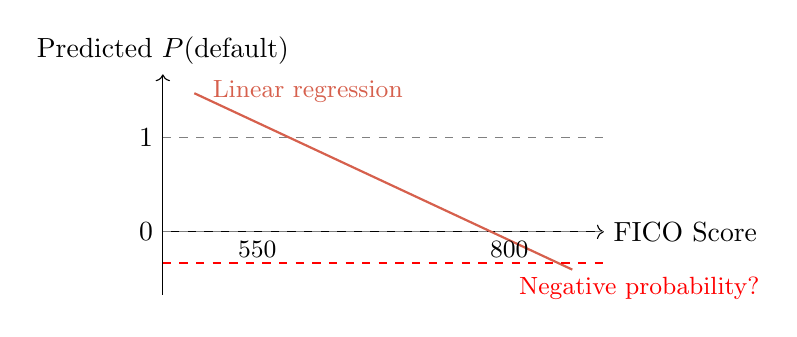
\begin{tikzpicture}[scale=0.8]
    % Axes
    \draw[->] (0,0) -- (7,0) node[right] {FICO Score};
    \draw[->] (0,-1) -- (0,2.5) node[above] {Predicted $P(\text{default})$};

    % Horizontal lines at 0 and 1
    \draw[dashed, gray] (0,0) -- (7,0);
    \draw[dashed, gray] (0,1.5) -- (7,1.5);
    \node[left] at (0,0) {0};
    \node[left] at (0,1.5) {1};

    % Linear regression line (goes outside [0,1])
    \draw[thick, AccentOrange] (0.5,2.2) -- (6.5,-0.6);
    \node[AccentOrange, above] at (2.3,1.9) {\small Linear regression};

    % Problem areas
    \draw[thick, red, dashed] (0,-0.5) -- (7,-0.5);
    \node[red, right] at (5.5,-0.9) {\small Negative probability?};

    % Axis labels
    \node[below] at (1.5,0) {\small 550};
    \node[below] at (5.5,0) {\small 800};
  \end{tikzpicture}
  \end{center}

  \vspace{0.3em}
  \textbf{The issue:} Linear regression can predict values outside $[0, 1]$
  \begin{itemize}
    \item A probability of $-0.2$ or $1.3$ does not make sense!
    \item We need methods designed for classification
  \end{itemize}
\end{frame}


\begin{frame}{Key Challenges in Credit Risk Prediction}

  \textbf{Before we dive into methods, let's understand the challenges:}

  \vspace{1em}
  \textbf{1. Class imbalance:} Defaults are relatively rare
  \begin{itemize}
    \item Typical portfolio: 10--20\% default rate
    \item A model that always predicts ``no default'' is 80--90\% accurate!
    \item But it's completely useless for identifying risky borrowers
  \end{itemize}

  \vspace{0.5em}
  \textbf{2. We need well-calibrated probabilities:}
  \begin{itemize}
    \item If model says ``15\% chance of default,'' roughly 15\% should actually default
    \item Critical for pricing and capital calculations
  \end{itemize}

  \vspace{0.5em}
  \textbf{3. Interpretability and fairness:}
  \begin{itemize}
    \item Regulators require explanations: ``Why was this loan denied?''
    \item Cannot discriminate based on protected characteristics
  \end{itemize}

  \vspace{0.5em}
  \textit{We'll address all of these on Wednesday's lecture.}
\end{frame}

%----------------------------------------------------------------------------------------
\section{Logistic Regression}
%----------------------------------------------------------------------------------------

\begin{frame}{The Core Idea: Predicting Probabilities}

  \textbf{What we want:} A model that predicts $P(\text{default} \mid \text{borrower characteristics})$

  \vspace{1em}
  \textbf{Requirements:}
  \begin{enumerate}
    \item Output must be between 0 and 1 (it's a probability!)
    \item Higher risk factors should increase the probability
    \item Should be interpretable (what drives the prediction?)
  \end{enumerate}

  \vspace{1em}
  \textbf{The solution: Logistic regression}
  \begin{itemize}
    \item Most widely used classification method
    \item Foundation of credit scoring for decades
    \item Interpretable: Can explain why a loan was approved/denied
  \end{itemize}

  \vspace{0.5em}
  \begin{block}{Key Insight}
    Logistic regression is like linear regression, but we transform the output to guarantee it's a valid probability
  \end{block}
\end{frame}

%----------------------------------------------------------------------------------------

\begin{frame}{From Linear to Logistic: The Sigmoid Function}

  \textbf{Linear regression:} $\widehat{y} = \beta_0 + \beta_1 x_1 + \beta_2 x_2 + \cdots$ \quad (can be any number)

  \vspace{0.5em}
  \textbf{Logistic regression:} Pass the linear combination through a \highlight{sigmoid function}

  \begin{center}
  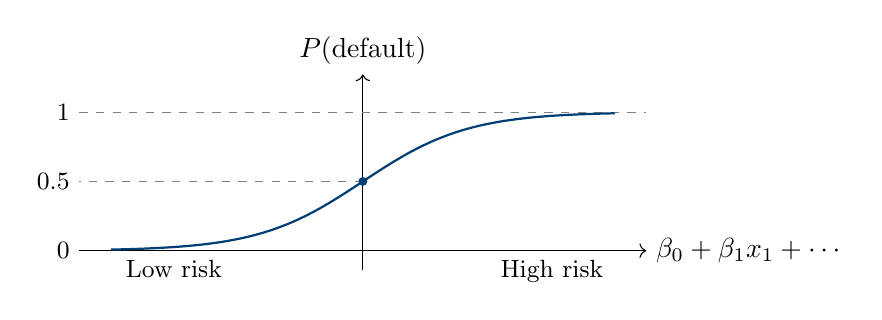
\begin{tikzpicture}[scale=0.8]
    \draw[->] (-4.5,0) -- (4.5,0) node[right] {$\beta_0 + \beta_1 x_1 + \cdots$};
    \draw[->] (0,-0.3) -- (0,2.8) node[above] {$P(\text{default})$};
    \draw[dashed, gray] (-4.5,2.2) -- (4.5,2.2);
    \node[left] at (-4.5,2.2) {\small 1};
    \node[left] at (-4.5,0) {\small 0};
    \draw[thick, ThemeBlue, domain=-4:4, samples=100] plot (\x, {2.2/(1+exp(-1.2*\x))});

    % Annotations
    \draw[dashed, gray] (0,1.1) -- (-4.5,1.1);
    \node[left] at (-4.5,1.1) {\small 0.5};
    \fill[ThemeBlue] (0,1.1) circle (2pt);

    % Labels for regions
    \node[below] at (-3,0) {\small Low risk};
    \node[below] at (3,0) {\small High risk};
  \end{tikzpicture}
  \end{center}

  \vspace{0.3em}
The sigmoid ``squashes'' any input into the range (0, 1):
  \[
  P(\text{default}) = \frac{1}{1 + e^{-(\beta_0 + \beta_1 x_1 + \cdots)}}
  \]
\end{frame}

%----------------------------------------------------------------------------------------

\begin{frame}{A Concrete Example}

  \textbf{Suppose our model learns these coefficients:}
  \begin{align*}
  \beta_0 &= 8 \quad \text{(intercept)} \\
  \beta_{\text{DTI}} &= 0.05 \quad \text{(debt-to-income ratio, in \%)} \\
  \beta_{\text{FICO}} &= -0.015 \quad \text{(credit score)}
  \end{align*}

  \vspace{0.5em}
  \textbf{Low-risk borrower:} DTI = 25\% and FICO = 750
  \begin{align*}
  \text{Linear part} &= 8 + 0.05 \times 25 + (-0.015) \times 750 = 8 + 1.25 - 11.25 = -2.0
  \end{align*}
  \[
  P(\text{default}) = \frac{1}{1 + e^{-(-2.0)}} = \frac{1}{1 + e^{2}} \approx \mathbf{0.12} \quad \text{(12\%)}
  \]

  \vspace{0.5em}
  \textbf{High-risk borrower:} DTI = 45\% and FICO = 620
  \begin{align*}
  \text{Linear part} &= 8 + 0.05 \times 45 + (-0.015) \times 620 = 8 + 2.25 - 9.30 = 0.95
  \end{align*}
  \[
  P(\text{default}) = \frac{1}{1 + e^{-0.95}} \approx \mathbf{0.72} \quad \text{(72\%)}
  \]
\end{frame}

%----------------------------------------------------------------------------------------

\begin{frame}{Interpreting the Coefficients: Odds Ratios}

  \textbf{The coefficients tell us how each variable affects default risk}

  \vspace{1em}
  \textbf{Interpretation via odds ratios:}
  \begin{itemize}
    \item For every 1-unit increase in $x_j$, the \highlight{odds of default} multiply by $e^{\beta_j}$
  \end{itemize}

  \vspace{0.5em}
  \textbf{Example:} If $\beta_{\text{DTI}} = 0.05$ (coefficient on debt-to-income ratio)
  \begin{itemize}
    \item $e^{0.05} \approx 1.05$
    \item Each 1\% point increase in DTI increases odds of default by $\sim$5\%
  \end{itemize}

  \vspace{1em}
  \textbf{This interpretability is valuable:}
  \begin{itemize}
    \item Regulators can understand what drives decisions
    \item Loan officers can explain denials to applicants
    \item Risk managers can identify key risk factors
  \end{itemize}
\end{frame}

%----------------------------------------------------------------------------------------

\begin{frame}{How Does Logistic Regression Learn? (Intuition)}

  \textbf{Linear regression:} We minimize squared errors (RSS)

  \vspace{0.5em}
  \textbf{Logistic regression:} We maximize the \highlight{likelihood} of observing our data

  \vspace{1em}
  \textbf{Intuition:}
  \begin{itemize}
    \item For borrowers who \textit{did} default: model should predict high probability
    \item For borrowers who \textit{didn't} default: model should predict low probability
    \item Find coefficients that make observed outcomes most ``likely''
  \end{itemize}

  \vspace{1em}
  \textbf{Technical detail (for the curious):}
  \begin{itemize}
    \item No closed-form solution (unlike OLS)
    \item Computer finds optimal coefficients iteratively
    \item sklearn handles this automatically, you don't need to worry about it!
  \end{itemize}
\end{frame}

%----------------------------------------------------------------------------------------

\begin{frame}{Regularization: Same Ideas as Linear Regression}

  \textbf{Problem:} With many predictors, logistic regression can overfit too!

  \vspace{1em}
  \textbf{Solution:} Add penalties, just like Ridge/Lasso

  \begin{center}
\renewcommand{\arraystretch}{1}
\resizebox{1\textwidth}{!}{\begin{tabular}{ll}
    \toprule
    \textbf{Penalty Type} & \textbf{Effect} \\
    \midrule
    L2 (Ridge) & Shrinks all coefficients toward zero \\
    L1 (Lasso) & Some coefficients become exactly zero (variable selection) \\
    Elastic Net & Combination of both \\
    \bottomrule
  \end{tabular}}
  \end{center}

  \vspace{1em}
  \textbf{Same intuition as Lecture 2:}
  \begin{itemize}
    \item Accept some bias to reduce variance
    \item Prevent model from fitting noise in the training data
    \item Tune the penalty strength using cross-validation
  \end{itemize}
\end{frame}

%----------------------------------------------------------------------------------------

\begin{frame}{Making Decisions: The Classification Threshold}

Logistic regression gives us probabilities of default.
\begin{itemize}
    \item How do we decide if a loan is predicted to default?
\end{itemize}

  \vspace{0.5em}
  \textbf{Simple rule:} Predict ``default'' if $P(\text{default}) > \tau$

  \vspace{0.5em}
  \begin{center}
  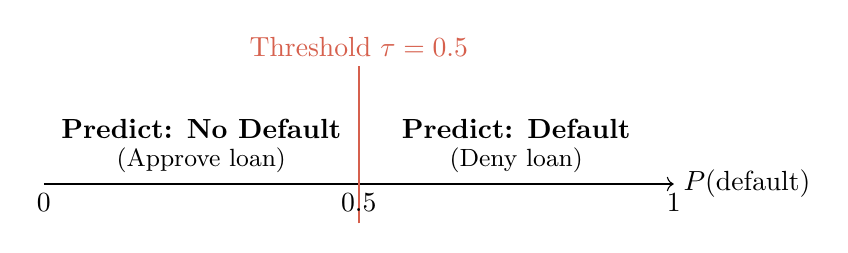
\begin{tikzpicture}[scale=1]
    \draw[->] (0,0) -- (8,0) node[right] {$P(\text{default})$};

    % Threshold line
    \draw[thick, AccentOrange] (4,-0.5) -- (4,1.5);
    \node[AccentOrange, above] at (4,1.5) {Threshold $\tau = 0.5$};

    % Regions
    \node at (2,0.7) {\textbf{Predict: No Default}};
    \node at (2,0.3) {\small (Approve loan)};
    \node at (6,0.7) {\textbf{Predict: Default}};
    \node at (6,0.3) {\small (Deny loan)};

    % Scale
    \node[below] at (0,0) {0};
    \node[below] at (4,0) {0.5};
    \node[below] at (8,0) {1};
  \end{tikzpicture}
  \end{center}

  \vspace{0.5em}
  \textbf{But $\tau = 0.5$ is not always the right choice!}
  \begin{itemize}
    \item If defaults are very costly, use lower threshold (be more cautious)
    \item If rejecting good borrowers is costly, use higher threshold
    \item We'll discuss threshold optimization on Wednesday
  \end{itemize}
\end{frame}

%----------------------------------------------------------------------------------------

\begin{frame}{The Decision Boundary}

  \textbf{The threshold creates a \highlight{decision boundary} in feature space}

  \vspace{0.5em}
  \begin{center}
  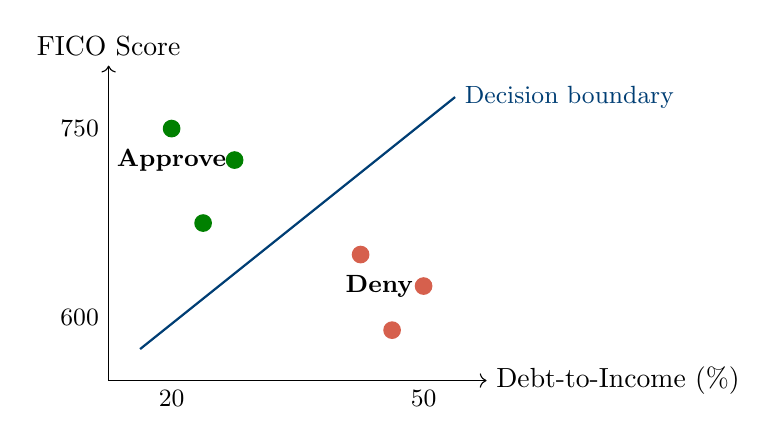
\begin{tikzpicture}[scale=0.8]
    % Axes
    \draw[->] (0,0) -- (6,0) node[right] {Debt-to-Income (\%)};
    \draw[->] (0,0) -- (0,5) node[above] {FICO Score};

    % Decision boundary (linear)
    \draw[thick, ThemeBlue] (0.5,0.5) -- (5.5,4.5);
    \node[ThemeBlue, right] at (5.5,4.5) {\small Decision boundary};

    % Regions
    \node at (1,3.5) {\small \textbf{Approve}};
    \node at (4.3,1.5) {\small \textbf{Deny}};

    % Some example points
    \fill[AccentGreen] (1,4) circle (4pt);
    \fill[AccentGreen] (2,3.5) circle (4pt);
    \fill[AccentGreen] (1.5,2.5) circle (4pt);
    \fill[AccentOrange] (4,2) circle (4pt);
    \fill[AccentOrange] (5,1.5) circle (4pt);
    \fill[AccentOrange] (4.5,0.8) circle (4pt);

    % Axis labels
    \node[below] at (1,0) {\small 20};
    \node[below] at (5,0) {\small 50};
    \node[left] at (0,1) {\small 600};
    \node[left] at (0,4) {\small 750};
  \end{tikzpicture}
  \end{center}

  \vspace{0.3em}
  \textbf{Key point:} Logistic regression produces a \highlight{linear} decision boundary
  \begin{itemize}
    \item Simple and interpretable
    \item But may not capture complex patterns in the data
  \end{itemize}
\end{frame}

%----------------------------------------------------------------------------------------

\begin{frame}{Logistic Regression: Summary}

  \textbf{What logistic regression does:}
  \begin{enumerate}
    \item Takes borrower characteristics as inputs
    \item Computes a weighted sum (like linear regression)
    \item Passes through sigmoid to get probability in $(0, 1)$
    \item Use threshold to convert probability to decision
  \end{enumerate}

  \vspace{1em}
  \textbf{Advantages:}
  \begin{itemize}
    \item Interpretable coefficients (odds ratios)
    \item Widely understood by regulators and practitioners
    \item Can add regularization to prevent overfitting
  \end{itemize}

  \vspace{0.5em}
  \textbf{Limitation:}
  \begin{itemize}
    \item Linear decision boundary --- may miss complex patterns
    \item Cannot automatically capture interactions between variables
  \end{itemize}
\end{frame}

%----------------------------------------------------------------------------------------
\section{Classification Trees}
%----------------------------------------------------------------------------------------

\begin{frame}{Trees for Classification: The Intuition}

  \textbf{Recall from Lecture 3:} Trees partition the data into regions

  \vspace{0.5em}
  \textbf{For regression:} Predict the average outcome in each region

  \textbf{For classification:} Predict the most common class (or class proportions)

  \vspace{1em}
  \begin{center}
  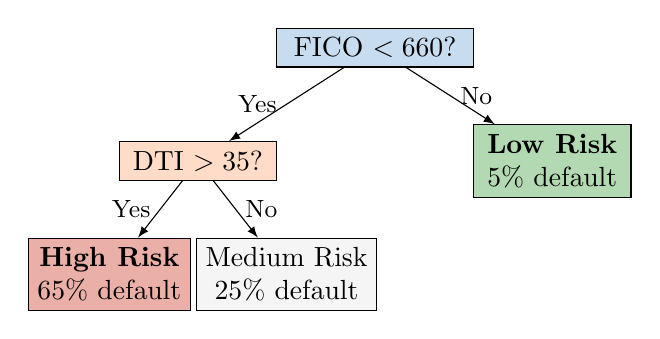
\begin{tikzpicture}[
    scale=0.9,
    every node/.style={align=center},
    level 1/.style={sibling distance=5cm, level distance=1.6cm},
    level 2/.style={sibling distance=2.5cm, level distance=1.6cm},
    edge from parent/.style={draw, -latex}
  ]
    \node[draw, rectangle, fill=LightBlue, minimum width=2.5cm] {FICO $< 660$?}
      child {
        node[draw, rectangle, fill=LightOrange, minimum width=2cm] {DTI $> 35$?}
          child {
            node[draw, rectangle, fill=AccentOrange!50, minimum width=1.5cm] {\textbf{High Risk}\\65\% default}
            edge from parent node[left, font=\small] {Yes}
          }
          child {
            node[draw, rectangle, fill=LightGray, minimum width=1.5cm] {Medium Risk\\25\% default}
            edge from parent node[right, font=\small] {No}
          }
        edge from parent node[left, font=\small] {Yes}
      }
      child {
        node[draw, rectangle, fill=AccentGreen!30, minimum width=2cm] {\textbf{Low Risk}\\5\% default}
        edge from parent node[right, font=\small] {No}
      };
  \end{tikzpicture}
  \end{center}

  \vspace{0.3em}
  \textbf{The tree discovers that:} Low FICO + high DTI = highest risk combination
\end{frame}

%----------------------------------------------------------------------------------------

\begin{frame}{How Trees Make Splits: Measuring ``Purity''}

  \textbf{Goal:} Each split should create more ``pure'' groups

  \vspace{0.5em}
  \textbf{Pure node:} All observations belong to same class (all default or all no-default)

  \vspace{1em}
  \textbf{How do we measure impurity?} The \highlight{Gini index}

  \vspace{0.5em}
  \textbf{Intuition:} If we randomly picked two loans from a region, how often would they have different outcomes?

  \vspace{0.5em}
  \begin{itemize}
    \item 50\% defaults, 50\% non-defaults: \highlight{High impurity} (Gini = 0.50)
    \item 90\% defaults, 10\% non-defaults: \highlight{Low impurity} (Gini = 0.18)
    \item 100\% defaults: \highlight{Pure} (Gini = 0)
  \end{itemize}

  \vspace{1em}
  \textbf{The algorithm:} Find the split that reduces impurity the most

  \vspace{0.5em}
  \textit{Technical note: ``Entropy'' is another common measure --- same idea, slightly different formula}
\end{frame}

%----------------------------------------------------------------------------------------

\begin{frame}{Classification Trees: Probability Outputs}

  \highlight{Trees can give us probabilities, not just class labels}

  \vspace{1em}
  \textbf{How?} Look at the proportion of each class in the leaf node

  \vspace{1em}
  \begin{center}
  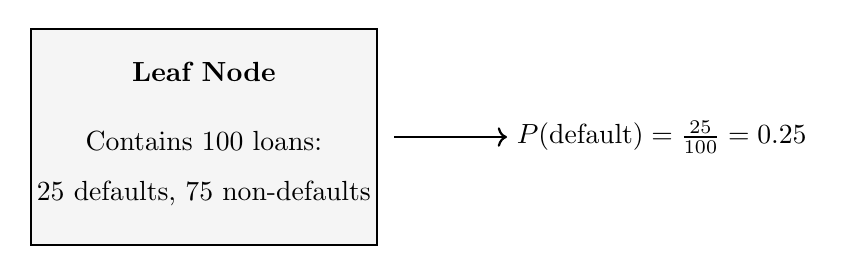
\begin{tikzpicture}[scale=1.1]
    % Leaf node
    \draw[thick, fill=LightGray] (0,0) rectangle (4,2.5);
    \node[font=\bfseries] at (2,2) {Leaf Node};

    % Contents
    \node at (2,1.2) {Contains 100 loans:};
    \node at (2,0.6) {25 defaults, 75 non-defaults};

    % Arrow and probability
    \draw[->, thick] (4.2,1.25) -- (5.5,1.25);
    \node[right] at (5.5,1.25) {$P(\text{default}) = \frac{25}{100} = 0.25$};
  \end{tikzpicture}
  \end{center}

  \vspace{1em}
  \textbf{Limitation:} Single trees produce ``coarse'' probabilities
  \begin{itemize}
    \item Only as many unique probability values as there are leaf nodes
    \item A tree with 10 leaves can only output 10 different probabilities
    \item Ensemble methods (next!) give smoother probability estimates
  \end{itemize}
\end{frame}

%----------------------------------------------------------------------------------------

\begin{frame}{Trees vs.\ Logistic Regression: What's Different?}

  \begin{center}
  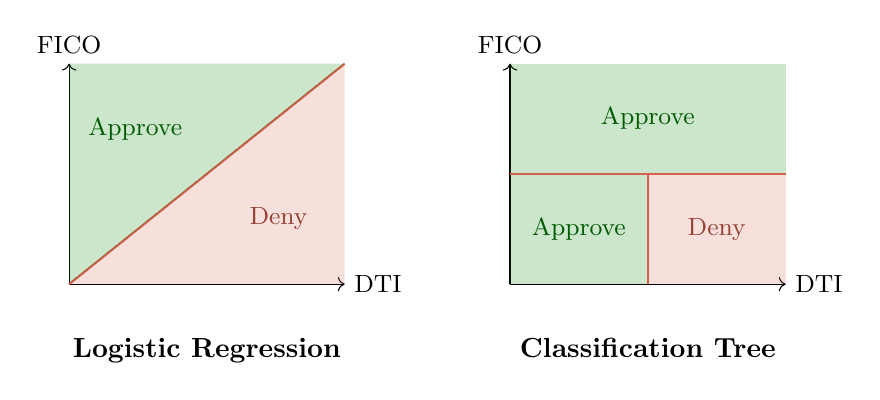
\begin{tikzpicture}[scale=0.7]
    % Logistic regression
    \begin{scope}[xshift=0cm]
      \draw[->] (0,0) -- (5,0) node[right] {\small DTI};
      \draw[->] (0,0) -- (0,4) node[above] {\small FICO};

      % Linear boundary
      \draw[thick, AccentOrange] (0,0) -- (5,4);

      % Shade regions
      \fill[AccentGreen, opacity=0.2] (0,0) -- (0,0) -- (0,4) -- (4,4) -- (5,4) -- cycle;
      \fill[AccentOrange, opacity=0.2] (0,0) -- (5,0) -- (5,4.5) -- (5,4) -- (5,4) -- cycle;

      % Labels
      \node[AccentGreen!70!black, font=\small] at (1.2,2.8) {Approve};
      \node[AccentOrange!70!black, font=\small] at (3.8,1.2) {Deny};

      \node[below] at (2.5,-0.8) {\textbf{Logistic Regression}};
    \end{scope}

    % Tree
    \begin{scope}[xshift=8cm]
      \draw[->] (0,0) -- (5,0) node[right] {\small DTI};
      \draw[->] (0,0) -- (0,4) node[above] {\small FICO};

      % Rectangular regions with shading
      \fill[AccentGreen, opacity=0.2] (0,2) rectangle (5,4);
      \fill[AccentGreen, opacity=0.2] (0,0) rectangle (2.5,2);
      \fill[AccentOrange, opacity=0.2] (2.5,0) rectangle (5,2);

      % Boundaries
      \draw[thick, AccentOrange] (0,2) -- (5,2);
      \draw[thick, AccentOrange] (2.5,0) -- (2.5,2);

      % Labels
      \node[AccentGreen!70!black, font=\small] at (2.5,3) {Approve};
      \node[AccentGreen!70!black, font=\small] at (1.25,1) {Approve};
      \node[AccentOrange!70!black, font=\small] at (3.75,1) {Deny};

      \node[below] at (2.5,-0.8) {\textbf{Classification Tree}};
    \end{scope}
  \end{tikzpicture}
  \end{center}

  \vspace{0.5em}
  \begin{columns}[T]
    \column{0.48\textwidth}
    \textbf{Logistic Regression:}
    \begin{itemize}
      \item Single straight-line boundary
      \item Same trade-off everywhere: higher FICO always compensates for higher DTI
    \end{itemize}

    \column{0.48\textwidth}
    \textbf{Classification Tree:}
    \begin{itemize}
      \item Axis-aligned splits (rectangles)
      \item Can capture \highlight{interactions}: high DTI only matters for default when FICO is low
    \end{itemize}
  \end{columns}
\end{frame}

%----------------------------------------------------------------------------------------

\begin{frame}{The Problem with Single Trees}

  \textbf{Recall from Lecture 3:} Single trees are \highlight{unstable}

  \vspace{1em}
  \begin{itemize}
    \item Small changes in data can produce completely different trees
    \item High variance in predictions
    \item Coarse probability estimates (limited unique values)
  \end{itemize}

  \vspace{1em}
  \textbf{The solution:} Build many trees and combine their predictions

  \vspace{0.5em}
  \begin{center}
  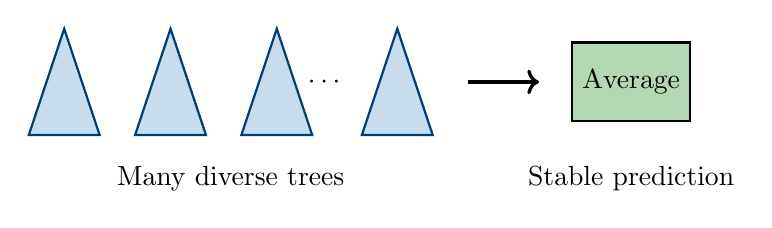
\begin{tikzpicture}[scale=0.9]
    % Multiple trees
    \foreach \x in {0, 1.5, 3} {
      \draw[thick, ThemeBlue, fill=LightBlue] (\x,0) -- (\x+0.5,1.5) -- (\x+1,0) -- cycle;
    }
    \node at (4.2,0.75) {$\cdots$};
    \draw[thick, ThemeBlue, fill=LightBlue] (4.7,0) -- (5.2,1.5) -- (5.7,0) -- cycle;

    % Arrow
    \draw[->, very thick] (6.2,0.75) -- (7.2,0.75);

    % Combined prediction
    \node[draw, thick, fill=AccentGreen!30, minimum width=1.5cm, minimum height=1cm] at (8.5,0.75) {Average};

    \node[below] at (2.85,-0.3) {Many diverse trees};
    \node[below] at (8.5,-0.3) {Stable prediction};
  \end{tikzpicture}
  \end{center}

  \vspace{0.5em}
  \textbf{Same ensemble ideas from Lecture 3 apply to classification!}
\end{frame}

%----------------------------------------------------------------------------------------

\begin{frame}{Random Forests for Classification}

  \textbf{Algorithm} (same as regression, different output):
  \begin{enumerate}
    \item Create $B$ bootstrap samples (random samples with replacement)
    \item Grow a tree on each sample, using random subset of features at each split
    \item Combine predictions from all trees
  \end{enumerate}

  \vspace{1em}
  \textbf{How to combine for classification:}

  \vspace{0.3em}
  \textbf{For class prediction:} Majority vote
  \begin{itemize}
    \item If 300 trees say ``default'' and 200 say ``no default'' $\Rightarrow$ predict ``default''
  \end{itemize}

  \vspace{0.3em}
  \textbf{For probability:} Average the probabilities
  \[
  P(\text{default}) = \frac{1}{B}\sum_{b=1}^{B} P_b(\text{default})
  \]

  \vspace{0.5em}
  \textbf{Key benefit:} Averaging produces \highlight{smoother} probability estimates
\end{frame}

%----------------------------------------------------------------------------------------

\begin{frame}{Why Averaging Helps: Smoother Probabilities}

  \begin{center}
  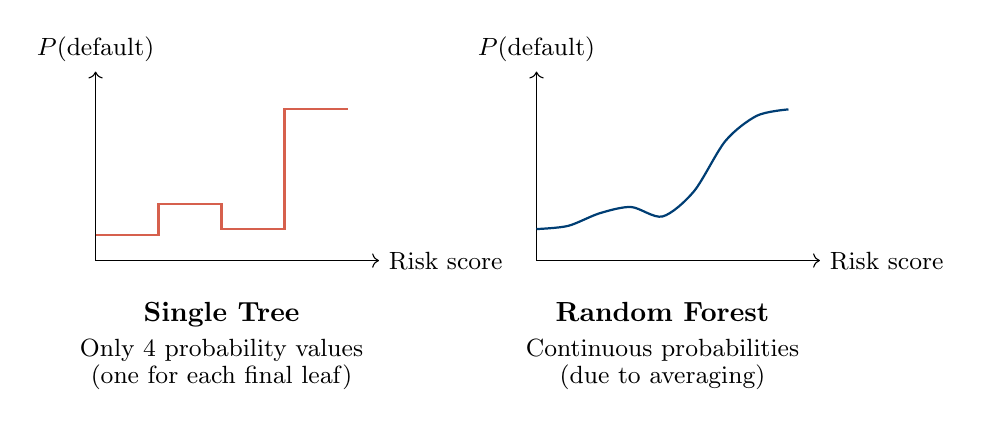
\begin{tikzpicture}[scale=0.8]
    % Single tree
    \begin{scope}[xshift=0cm]
      \draw[->] (0,0) -- (4.5,0) node[right] {\small Risk score};
      \draw[->] (0,0) -- (0,3) node[above] {\small $P(\text{default})$};

      % Step function
      \draw[thick, AccentOrange] (0,0.4) -- (1,0.4) -- (1,0.9) -- (2,0.9) --
        (2,0.5) -- (3,0.5) -- (3,2.4) -- (4,2.4);

      \node[below] at (2,-0.5) {\textbf{Single Tree}};
      \node[below] at (2,-1.1) {\small Only 4 probability values};
      \node[below] at (2,-1.5) {\small (one for each final leaf)};

    \end{scope}

    % Random Forest
    \begin{scope}[xshift=7cm]
      \draw[->] (0,0) -- (4.5,0) node[right] {\small Risk score};
      \draw[->] (0,0) -- (0,3) node[above] {\small $P(\text{default})$};

      % Smooth curve
      \draw[thick, ThemeBlue, smooth] plot coordinates {
        (0,0.5) (0.5,0.55) (1,0.75) (1.5,0.85) (2,0.7) (2.5,1.1) (3,1.9) (3.5,2.3) (4,2.4)
      };

      \node[below] at (2,-0.5) {\textbf{Random Forest}};
      \node[below] at (2,-1.1) {\small Continuous probabilities};            \node[below] at (2,-1.5) {\small (due to averaging)};

    \end{scope}
  \end{tikzpicture}
  \end{center}

  \vspace{0.5em}
  \textbf{Why this matters for credit risk:}
  \begin{itemize}
    \item Better differentiation between borrowers
    \item More accurate risk-based pricing
    \item Smoother ranking of applicants by risk level
  \end{itemize}
\end{frame}

%----------------------------------------------------------------------------------------

\begin{frame}{Gradient Boosting for Classification}

  \textbf{Same sequential idea as Lecture 3:}
  \begin{enumerate}
    \item Start with a simple prediction
    \item Build trees that focus on \highlight{mistakes} from previous trees
    \item Combine with shrinkage (learning slowly)
  \end{enumerate}

  \vspace{1em}
  \textbf{For classification:} Trees try to improve probability estimates
  \begin{itemize}
    \item Focus on loans where current probability is most wrong
    \item Gradually refine the predictions
  \end{itemize}

  \vspace{1em}
  \textbf{Key difference from Random Forest:}
  \begin{itemize}
    \item RF: Trees are independent (parallel)
    \item Boosting: Each tree depends on previous ones (sequential)
    \item Boosting often achieves better accuracy, but needs more tuning
  \end{itemize}
\end{frame}

%----------------------------------------------------------------------------------------

\begin{frame}{Handling Class Imbalance}

  \textbf{The problem:} If only 15\% of loans default...
  \begin{itemize}
    \item Model can achieve 85\% accuracy by always predicting ``no default''
    \item But this is useless for identifying risky borrowers!
  \end{itemize}

  \vspace{0.5em}
  \textbf{The intuition:} Make errors on defaults more ``costly'' during training

  \begin{center}
  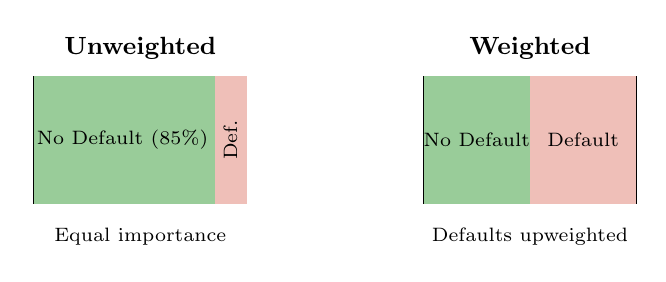
\begin{tikzpicture}[scale=0.9]
    % Unweighted
    \begin{scope}[xshift=0cm]
      \node[font=\small\bfseries] at (1.5,2.2) {Unweighted};
      \draw (0,0) rectangle (3,1.8);
      \fill[AccentGreen!40] (0,0) rectangle (2.55,1.8);
      \fill[AccentOrange!40] (2.55,0) rectangle (3,1.8);
      \node[font=\scriptsize] at (1.25,0.9) {No Default (85\%)};
      \node[font=\scriptsize] at (2.77,0.9) {\rotatebox{90}{Def.}};
      \node[font=\scriptsize, below] at (1.5,-0.2) {Equal importance};
    \end{scope}

    % Weighted
    \begin{scope}[xshift=5.5cm]
      \node[font=\small\bfseries] at (1.5,2.2) {Weighted};
      \draw (0,0) rectangle (3,1.8);
      \fill[AccentGreen!40] (0,0) rectangle (1.5,1.8);
      \fill[AccentOrange!40] (1.5,0) rectangle (3,1.8);
      \node[font=\scriptsize] at (0.75,0.9) {No Default};
      \node[font=\scriptsize] at (2.25,0.9) {Default};
      \node[font=\scriptsize, below] at (1.5,-0.2) {Defaults upweighted};
    \end{scope}
  \end{tikzpicture}
  \end{center}

 \vspace{-0.3em}
  \textbf{In sklearn:}
  \begin{itemize}
    \item \texttt{class\_weight='balanced'} --- adjusts weights inversely to class frequency.
    \item \textbf{Example:} 85\% No Default, 15\% Default.
    \item Weights: No Default $\approx 0.59$, Default $\approx 3.33$.
    \item Each default loan counts $\sim$5.6x more in the loss.
  \end{itemize}
\end{frame}

%----------------------------------------------------------------------------------------
\section{The LendingClub Application}
%----------------------------------------------------------------------------------------

\begin{frame}{Recap: What We Learned in Part I}

  \textbf{Classification methods for credit risk:}
  \begin{itemize}
    \item \textbf{Logistic regression:} Interpretable, linear decision boundary
    \item \textbf{Classification trees:} Automatic interactions, rectangular regions
    \item \textbf{Random Forests:} Variance reduction, smoother probabilities
    \item \textbf{Gradient Boosting:} Often best accuracy, needs tuning
  \end{itemize}

  \vspace{1em}
  \textbf{All methods give us:}
  \begin{enumerate}
    \item Class predictions (default / no default)
    \item Probability estimates: $\widehat{P}(\text{default} \mid X)$
  \end{enumerate}

  \vspace{1em}
  \begin{block}{Today's Questions}
    We've trained our models. Now what? How do we \highlight{evaluate} them and turn predictions into \highlight{business decisions}?
  \end{block}
\end{frame}

%----------------------------------------------------------------------------------------

\begin{frame}{The LendingClub Dataset}

  \textbf{Our application:} Peer-to-peer lending platform

  \vspace{0.5em}
  \begin{columns}[T]
    \column{0.48\textwidth}
    \textbf{Features available:}
    \begin{itemize}
      \item Loan amount, interest rate
      \item Annual income
      \item Employment length
      \item Debt-to-income ratio
      \item Credit history length
      \item Number of open accounts
      \item Revolving balance \& utilization
      \item Past delinquencies
      \item Home ownership, loan purpose
    \end{itemize}

    \column{0.48\textwidth}
    \textbf{Target:}
    \begin{itemize}
      \item Default (1) vs.\ No Default (0)
    \end{itemize}

    \vspace{0.5em}
    \textbf{Sample:}
    \begin{itemize}
      \item $\sim$1.2mln loans
      \item Default rate: $\sim$20\%
    \end{itemize}

    \vspace{0.5em}
    \textbf{Business goal:}
    \begin{itemize}
      \item Decide: approve or deny?
      \item Set appropriate interest rate
    \end{itemize}
  \end{columns}
\end{frame}

%----------------------------------------------------------------------------------------

\begin{frame}{We've Trained Three Models}

  \textbf{Setup:}
  \begin{itemize}
    \item 70\% training / 15\% validation / 15\% test split
    \item Used \texttt{class\_weight='balanced'} to handle imbalance
    \item Tuned hyperparameters on validation set
  \end{itemize}

  \vspace{1em}
  \textbf{Models:}
  \begin{enumerate}
    \item \textbf{Logistic Regression} (L2 regularized) --- our interpretable baseline
    \item \textbf{Random Forest} (500 trees, max\_depth=10)
    \item \textbf{XGBoost} (with early stopping)
  \end{enumerate}

  \vspace{1em}
  \textbf{Now we need to answer:}
  \begin{itemize}
    \item Which model is ``best''?
    \item How do we measure ``best''?
    \item What threshold should we use for decisions?
  \end{itemize}
\end{frame}

%----------------------------------------------------------------------------------------

\begin{frame}{The Business Context}

  \textbf{Why do we care about these predictions?}

  \vspace{1em}
  \textbf{Decisions that depend on default probabilities:}
  \begin{enumerate}
    \item \highlight{Approve or deny} the loan application
    \item \highlight{Set the interest rate} (higher risk $\Rightarrow$ higher rate)
    \item \highlight{Determine loan limits}
    \item \highlight{Calculate expected losses} for the portfolio
    \item \highlight{Regulatory capital} requirements
  \end{enumerate}

  \vspace{1em}
  \textbf{This means we need:}
  \begin{itemize}
    \item A model that \highlight{ranks} borrowers correctly (separates good from bad)
    \item A way to choose the right \highlight{decision threshold}
    \item \highlight{Well-calibrated} probabilities (if using for pricing)
  \end{itemize}
\end{frame}

%----------------------------------------------------------------------------------------
\section{Model Evaluation}
%----------------------------------------------------------------------------------------

\begin{frame}{Why Accuracy Is Misleading}

  \textbf{Accuracy:} Fraction of correct predictions
  \[
  \text{Accuracy} = \frac{\text{Correct predictions}}{\text{Total predictions}}
  \]

  \vspace{0.3em}
  \textbf{The problem with imbalanced data:}

  \vspace{0.3em}
  \begin{center}
  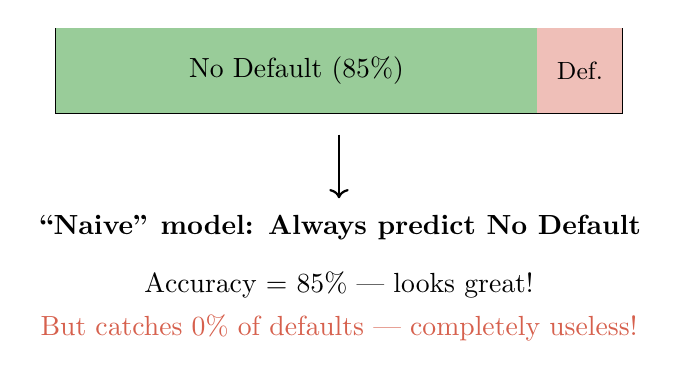
\begin{tikzpicture}[scale=0.9]
    % Data distribution
    \draw (0,0) rectangle (8,1.2);
    \fill[AccentGreen!40] (0,0) rectangle (6.8,1.2);
    \fill[AccentOrange!40] (6.8,0) rectangle (8,1.2);

    \node at (3.4,0.6) {No Default (85\%)};
    \node at (7.4,0.6) {\small Def.};

    % Arrow
    \draw[->, thick] (4,-0.3) -- (4,-1.2);

    % Naive model
    \node[below] at (4,-1.3) {\textbf{``Naive'' model: Always predict No Default}};
    \node[below] at (4,-2.1) {Accuracy = 85\% --- looks great!};
    \node[below, AccentOrange] at (4,-2.7) {But catches 0\% of defaults --- completely useless!};
  \end{tikzpicture}
  \end{center}

  \textbf{Lesson:} With imbalanced classes, we need better metrics
\end{frame}

%----------------------------------------------------------------------------------------

\begin{frame}{The Confusion Matrix}

  \textbf{Foundation:} Count predictions by actual vs.\ predicted class

  \begin{center}
  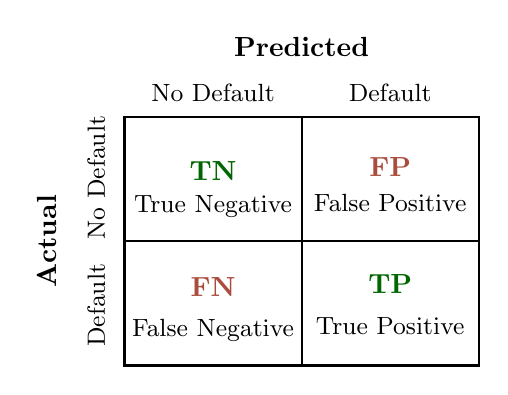
\begin{tikzpicture}[scale=0.9]
    % Matrix
    \draw[thick] (0,0) rectangle (5,3.5);
    \draw[thick] (2.5,0) -- (2.5,3.5);
    \draw[thick] (0,1.75) -- (5,1.75);

    % Headers
    \node[font=\bfseries] at (2.5,4.5) {Predicted};
    \node at (1.25,3.85) {\small No Default};
    \node at (3.75,3.85) {\small Default};

    \node[font=\bfseries, rotate=90] at (-1.1,1.75) {Actual};
    \node[rotate=90] at (-0.4,2.65) {\small No Default};
    \node[rotate=90] at (-0.4,0.85) {\small Default};

    % Cells
    \node[AccentGreen!80!black, font=\bfseries] at (1.25,2.75) {TN};
    \node[font=\small] at (1.25,2.25) {True Negative};

    \node[AccentOrange!80!black, font=\bfseries] at (3.75,2.8) {FP};
    \node[font=\small] at (3.75,2.3) {False Positive};

    \node[AccentOrange!80!black, font=\bfseries] at (1.25,1.1) {FN};
    \node[font=\small] at (1.25,0.5) {False Negative};

    \node[AccentGreen!80!black, font=\bfseries] at (3.75,1.15) {TP};
    \node[font=\small] at (3.75,0.55) {True Positive};
  \end{tikzpicture}
  \end{center}

  \vspace{0.5em}
  \textbf{Credit risk interpretation:}
  \begin{itemize}
    \item \textbf{FP} (False Positive): Denied a good borrower $\rightarrow$ lost business
    \item \textbf{FN} (False Negative): Approved a defaulter $\rightarrow$ lost money
  \end{itemize}
\end{frame}

%----------------------------------------------------------------------------------------

\begin{frame}{The Confusion Matrix: Our LendingClub Results}

  \textbf{Logistic regression predictions} (+188k test loans, threshold = 0.5):

  \vspace{0.5em}
   \begin{center}
  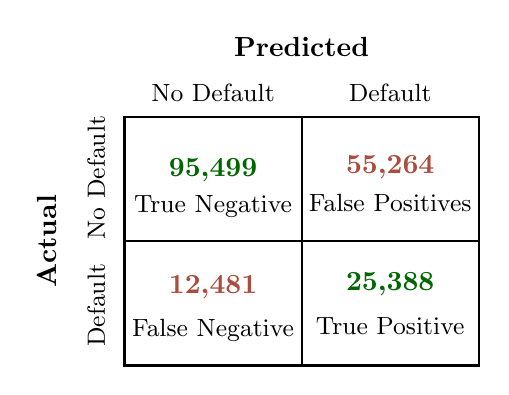
\begin{tikzpicture}[scale=0.9]
    % Matrix
    \draw[thick] (0,0) rectangle (5,3.5);
    \draw[thick] (2.5,0) -- (2.5,3.5);
    \draw[thick] (0,1.75) -- (5,1.75);

    % Headers
    \node[font=\bfseries] at (2.5,4.5) {Predicted};
    \node at (1.25,3.85) {\small No Default};
    \node at (3.75,3.85) {\small Default};

    \node[font=\bfseries, rotate=90] at (-1.1,1.75) {Actual};
    \node[rotate=90] at (-0.4,2.65) {\small No Default};
    \node[rotate=90] at (-0.4,0.85) {\small Default};

    % Cells
    \node[AccentGreen!80!black, font=\bfseries] at (1.25,2.75) {95,499};
    \node[font=\small] at (1.25,2.25) {True Negative};

    \node[AccentOrange!80!black, font=\bfseries] at (3.75,2.8) {55,264};
    \node[font=\small] at (3.75,2.3) {False Positives};

    \node[AccentOrange!80!black, font=\bfseries] at (1.25,1.1) {12,481};
    \node[font=\small] at (1.25,0.5) {False Negative};

    \node[AccentGreen!80!black, font=\bfseries] at (3.75,1.15) {25,388};
    \node[font=\small] at (3.75,0.55) {True Positive};
  \end{tikzpicture}
  \end{center}

  \vspace{0.3em}
  \textbf{Reading this:}
  \begin{itemize}
    \item \textbf{FP = 55,264}: Good borrowers we would have wrongly denied (lost business)
    \item \textbf{FN = 12,481}: Defaulters we would have approved (lost money!)
  \end{itemize}
\end{frame}

%----------------------------------------------------------------------------------------

\begin{frame}{Precision: How Reliable Are Our ``Deny'' Decisions?}

  \textbf{Precision:} Of those we predict as default, how many actually default?

  \[
  \text{Precision} = \frac{TP}{TP + FP} = \frac{\text{Correctly predicted defaults}}{\text{All predicted defaults}}
  \]

  \vspace{0.5em}
  \textbf{From our Logistic regression confusion matrix:}
  \[
  \text{Precision} = \frac{25,388}{25,388 + 55,264} = \frac{25,388}{80,652} = 31.5\%
  \]

  \vspace{1em}
  \textbf{Interpretation:}
  \begin{itemize}
    \item We flagged 80,652 loans as high-risk
    \item Only 31.5\% of them actually defaulted
    \item The other 68.5\% were \highlight{good borrowers we would have turned away}
  \end{itemize}

  \vspace{0.5em}
  \textbf{When precision matters:} When denying good borrowers is costly (lost profit)
\end{frame}

%----------------------------------------------------------------------------------------

\begin{frame}{Recall: How Many Defaults Did We Catch?}

  \textbf{Recall:} Of all actual defaults, what fraction did we identify?

  \[
  \text{Recall} = \frac{TP}{TP + FN} = \frac{\text{Correctly predicted defaults}}{\text{All actual defaults}}
  \]

  \vspace{0.5em}
  \textbf{From our Logistic regression confusion matrix:}
  \[
  \text{Recall} = \frac{25,388}{25,388 + 12,481} = \frac{25,388}{37,869} = 67.1\%
  \]

  \vspace{1em}
  \textbf{Interpretation:}
  \begin{itemize}
    \item There were 37,869 loans that actually defaulted
    \item We correctly identified 67.1\% of them
    \item But \highlight{32.9\% of defaults slipped through} --- we approved them!
  \end{itemize}

  \vspace{0.5em}
  \textbf{When recall matters:} When approving defaulters is costly (lost principal)
\end{frame}

%----------------------------------------------------------------------------------------

\begin{frame}{The Precision-Recall Trade-off}

  \textbf{You can't maximize both simultaneously!}

  \vspace{0.5em}
  \begin{center}
  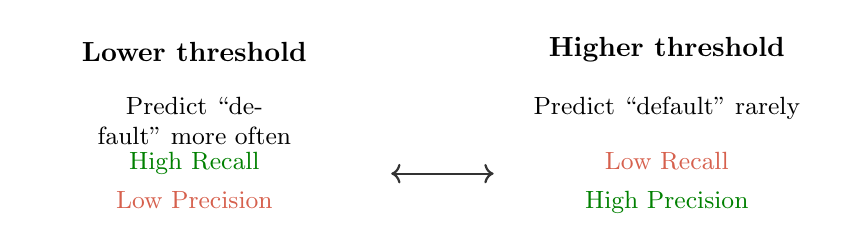
\begin{tikzpicture}[scale=1]
    % Low threshold
    \node[above] at (0.5,0.5) {\textbf{Lower threshold}};
    \node[below, font=\small, text width=4cm, align=center] at (0.5,0.3) {Predict ``default'' more often};
    \node[below, font=\small, AccentGreen] at (0.5,-0.4) {High Recall};
    \node[below, font=\small, AccentOrange] at (0.5,-0.9) {Low Precision};

    % High threshold
    \node[above] at (6.5,0.5) {\textbf{Higher threshold}};
    \node[below, font=\small, text width=3.5cm, align=center] at (6.5,0.3) {Predict ``default'' rarely};
    \node[below, font=\small, AccentOrange] at (6.5,-0.4) {Low Recall};
    \node[below, font=\small, AccentGreen] at (6.5,-0.9) {High Precision};

    % Arrow
    \draw[<->, thick, DarkGray] (3,-0.8) -- (4.3,-0.8);
  \end{tikzpicture}
  \end{center}

  \vspace{1em}
  \textbf{The core tension:}
  \begin{itemize}
    \item Lower threshold $\Rightarrow$ catch more defaults, but also deny more good borrowers
    \item Higher threshold $\Rightarrow$ fewer false alarms, but miss more defaults
  \end{itemize}

  \vspace{0.5em}
  \textbf{Which matters more?} Depends on the business costs!
\end{frame}

%----------------------------------------------------------------------------------------

\begin{frame}{F1 Score: Balancing Precision and Recall}

  \textbf{Problem:} How do we compare models when one has higher precision but lower recall?

  \vspace{1em}
  \textbf{F1 Score:} The harmonic mean of precision and recall
  \[
  F_1 = 2 \times \frac{\text{Precision} \times \text{Recall}}{\text{Precision} + \text{Recall}}
  \]

  \vspace{0.5em}
  \textbf{Our Logistic regression model:}
  \[
  F_1 = 2 \times \frac{0.315 \times 0.671}{0.315 + 0.671} = 2 \times \frac{0.211}{0.985} = 0.428
  \]

  \vspace{1em}
  \textbf{Why harmonic mean?}
  \begin{itemize}
    \item Penalizes extreme imbalances
    \item If either precision or recall is very low, F1 will be low
    \item Requires \textit{both} to be good to score well
  \end{itemize}
\end{frame}

%----------------------------------------------------------------------------------------

\begin{frame}{Comparing Our Models: Precision, Recall, F1}

  \textbf{Results at threshold = 0.5:}

  \vspace{0.5em}
  \begin{center}
  \begin{tabular}{lcccc}
    \toprule
    \textbf{Model} & \textbf{Precision} & \textbf{Recall} & \textbf{F1} & \textbf{Accuracy} \\
    \midrule
Logistic Regression	&0.315	&0.670	&0.428 & 0.641\\
Random Forest	&0.307	&0.686	&0.424 & 0.623\\
XGBoost	&0.323	&0.676	&0.437 & 0.651\\
    \bottomrule
  \end{tabular}
  \end{center}

  \vspace{1em}
  \textbf{Observations:}
  \begin{itemize}
    \item XGBoost has the best F1 score (0.437)
    \item All models catch only 67--68\% of defaults (recall)
    \item About 30\% of ``deny'' decisions would be wrong (precision $\approx$ 0.30)
  \end{itemize}

  \vspace{0.5em}
  \textbf{Question:} Can we compare models \textit{across all thresholds}?
\end{frame}

%----------------------------------------------------------------------------------------

\begin{frame}{ROC Curve: Evaluating Across All Thresholds}

  \textbf{Idea:} Plot the trade-off as we vary the threshold from 0 to 1

  \vspace{0.3em}
  \begin{columns}[T]
    \column{0.55\textwidth}
    \textbf{Definitions:}
    \begin{align*}
    \text{True Positive Rate} &= \frac{TP}{TP + FN}\\[0.5em]
    \text{False Positive Rate} &= \frac{FP}{FP + TN}
    \end{align*}

    \vspace{0.5em}
    \textbf{Interpretation:}
    \begin{itemize}
      \item TPR: Fraction of defaults we catch
      \item FPR: Fraction of good loans we wrongly flag
    \end{itemize}

\column{0.4\textwidth}
    \begin{center}
    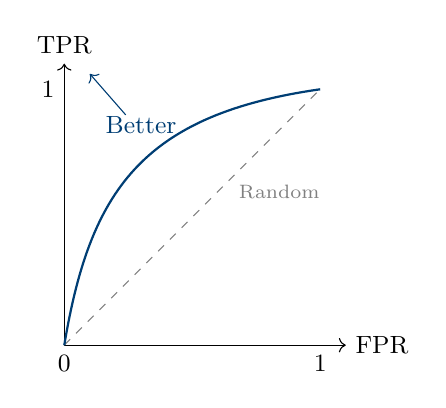
\begin{tikzpicture}[scale=0.65]
      % Axes
      \draw[->] (0,0) -- (5.5,0) node[right] {\small FPR};
      \draw[->] (0,0) -- (0,5.5) node[above] {\small TPR};

      % Diagonal (random)
      \draw[dashed, gray] (0,0) -- (5,5);
      \node[gray, font=\scriptsize] at (4.2,3) {Random};

      % ROC curve
      \draw[thick, ThemeBlue] (0,0) .. controls (0.5,3) and (1.5,4.5) .. (5,5);

      % Labels
      \node[below] at (0,0) {\small 0};
      \node[below] at (5,0) {\small 1};
      \node[left] at (0,5) {\small 1};

      % Annotation
      \node[ThemeBlue, font=\small] at (1.5,4.3) {Better};
      \draw[->, ThemeBlue] (1.2,4.5) -- (0.5,5.3);
    \end{tikzpicture}
    \end{center}
  \end{columns}

  \vspace{1em}
 \textbf{What makes a good ROC curve?}
  \begin{itemize}
    \item Curves toward the \highlight{top-left corner} (high TPR, low FPR)
    \item Diagonal line = random guessing (no predictive power)
  \end{itemize}
\end{frame}

%----------------------------------------------------------------------------------------

\begin{frame}{Our Models: ROC Curves}

  \begin{center}
  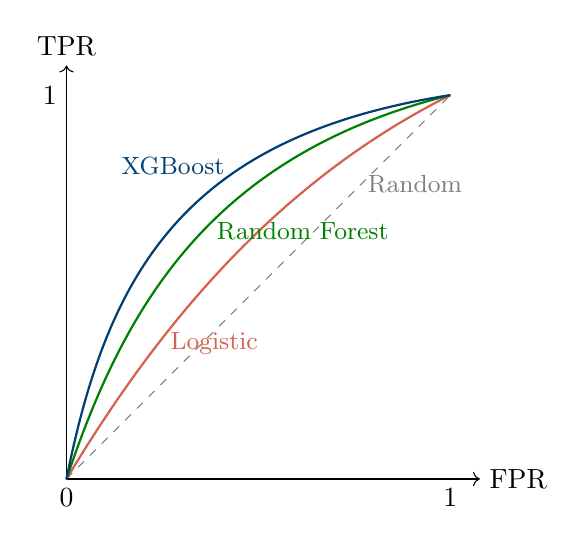
\begin{tikzpicture}[scale=0.75]
    % Axes
    \draw[->] (0,0) -- (7,0) node[right] {FPR};
    \draw[->] (0,0) -- (0,7) node[above] {TPR};

    % Diagonal
    \draw[dashed, gray] (0,0) -- (6.5,6.5);
    \node[gray, font=\small] at (5.9,5) {Random};

    % Logistic Regression (AUC = 0.72)
    \draw[thick, AccentOrange] (0,0) .. controls (1.5,2.5) and (3.5,5) .. (6.5,6.5);

    % Random Forest (AUC = 0.76)
    \draw[thick, AccentGreen] (0,0) .. controls (1,3) and (2.5,5.5) .. (6.5,6.5);

    % XGBoost (AUC = 0.79)
    \draw[thick, ThemeBlue] (0,0) .. controls (0.7,3.5) and (2,5.8) .. (6.5,6.5);

    % Legend
    \node[AccentOrange, font=\small] at (2.5,2.3) {Logistic};
    \node[AccentGreen, font=\small] at (4,4.2) {Random Forest};
    \node[ThemeBlue, font=\small] at (1.8,5.3) {XGBoost};

    % Axis labels
    \node[below] at (0,0) {0};
    \node[below] at (6.5,0) {1};
    \node[left] at (0,6.5) {1};
  \end{tikzpicture}
  \end{center}

  \vspace{0.3em}
  \textbf{Reading this:} XGBoost dominates at almost every threshold
\end{frame}

%----------------------------------------------------------------------------------------

\begin{frame}{AUC: A Single Number Summary}

  \begin{columns}[T]
    \column{0.52\textwidth}
    \textbf{AUC} = Area Under the ROC Curve

    \vspace{0.5em}
    \begin{center}
    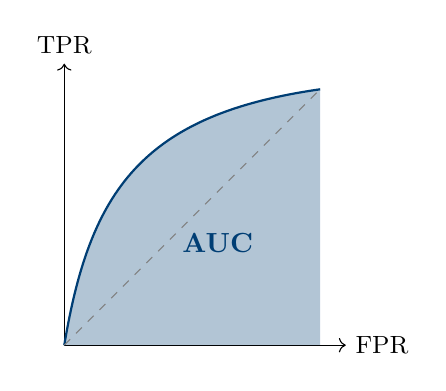
\begin{tikzpicture}[scale=0.65]
      % Axes
      \draw[->] (0,0) -- (5.5,0) node[right] {\small FPR};
      \draw[->] (0,0) -- (0,5.5) node[above] {\small TPR};

      % Shaded area
      \fill[ThemeBlue, opacity=0.3] (0,0) .. controls (0.5,3) and (1.5,4.5) .. (5,5) -- (5,0) -- cycle;

      % ROC curve
      \draw[thick, ThemeBlue] (0,0) .. controls (0.5,3) and (1.5,4.5) .. (5,5);

      % Diagonal
      \draw[dashed, gray] (0,0) -- (5,5);

      % AUC label
      \node[ThemeBlue, font=\bfseries] at (3,2) {AUC};
    \end{tikzpicture}
    \end{center}

    \column{0.48\textwidth}
    \textbf{Interpretation:}
    \begin{itemize}
      \item AUC = 0.5: Random guessing
      \item AUC = 1.0: Perfect
      \item AUC = 0.73: Good (our XGBoost)
    \end{itemize}

    \vspace{0.5em}
    \textbf{Intuitive meaning:}

If we randomly pick one defaulter and one non-defaulter from our test set, there's a 73\% chance the model correctly ranks the defaulter as riskier.
  \end{columns}

  \vspace{1em}
  \textbf{LendingClub results:}
  \begin{center}
  \begin{tabular}{lc}
    Logistic Regression & AUC = 0.709 \\
    Random Forest & AUC = 0.707 \\
    XGBoost & AUC = 0.722 \\
  \end{tabular}
  \end{center}
\end{frame}

%----------------------------------------------------------------------------------------

\begin{frame}{Which Metric Should We Use?}

  \begin{center}
  \begin{tabular}{ll}
    \toprule
    \textbf{Situation} & \textbf{Focus on} \\
    \midrule
    Comparing models (threshold not yet chosen) & \textbf{AUC} \\
    \addlinespace
    Limited capital, can't afford bad loans & \textbf{Precision} \\
    \addlinespace
    Must identify risky borrowers (regulatory) & \textbf{Recall} \\
    \addlinespace
    Need balance between both errors & \textbf{F1 Score} \\
    \bottomrule
  \end{tabular}
  \end{center}

  \vspace{1em}
  \begin{block}{Key Insight}
    There's no single ``best'' metric --- it depends on the \highlight{costs of different errors}
  \end{block}
\end{frame}

%----------------------------------------------------------------------------------------
\section{Threshold Optimization}
%----------------------------------------------------------------------------------------

\begin{frame}{Why 0.5 Is Usually Wrong}

  \textbf{Default threshold:} Predict ``default'' if $P(\text{default}) > 0.5$

  \vspace{1em}
  \textbf{This assumes:}
  \begin{itemize}
    \item Cost of denying a good borrower = Cost of approving a defaulter
  \end{itemize}

  \vspace{1em}
  \textbf{But in reality:}

  \vspace{0.3em}
  \begin{center}
  \begin{tabular}{lc}
    \toprule
    \textbf{Error Type} & \textbf{Typical Cost} \\
    \midrule
    False Positive (deny good borrower) & Lost profit: \pounds 500 \\
    False Negative (approve defaulter) & Lost principal: \pounds 5,000 \\
    \bottomrule
  \end{tabular}
  \end{center}

  \vspace{1em}
  \textbf{Defaults are 10$\times$ more costly!}

  \vspace{0.3em}
  \textbf{Implication:} We should use a \highlight{lower threshold} to be more cautious
\end{frame}

%----------------------------------------------------------------------------------------

\begin{frame}{Cost-Sensitive Decision Making}

  \textbf{Framework:} Choose threshold to minimize expected cost

  \vspace{1em}
  \textbf{Define:}
  \begin{itemize}
    \item $C_{FP}$ = \pounds 500 (cost of denying a good borrower)
    \item $C_{FN}$ = \pounds 5,000 (cost of approving a defaulter)
  \end{itemize}

  \vspace{0.5em}
  \textbf{Total expected cost:}
  \[
  \text{Total Cost} = C_{FP} \times \#FP + C_{FN} \times \#FN
  \]

  \vspace{1em}
  \textbf{Trade-off:}
  \begin{itemize}
    \item Lower threshold $\Rightarrow$ more FP (deny good borrowers), fewer FN (catch more defaults)
    \item Higher threshold $\Rightarrow$ fewer FP, more FN
  \end{itemize}

  \vspace{0.5em}
  \textbf{Goal:} Find the threshold that minimizes total cost
\end{frame}

%----------------------------------------------------------------------------------------

\begin{frame}{Finding the Optimal Threshold}

  \textbf{Our XGBoost model at different thresholds:}

  \vspace{0.5em}
  \begin{center}
  \begin{tabular}{ccccc}
    \toprule
    \textbf{Threshold} & \textbf{FP} & \textbf{FN} & \textbf{Total Cost} & \\
    \midrule
    0.50 & 53,588 & 12,263 & \pounds 72.0m & \\
    0.40 & 81,325 & 6,367 & \pounds 48.1m & \\
    0.30 & 108,799 & 2,677 & \pounds 35.1m & \\
    0.20 & 131,401 & 735 & \pounds 30.0m & \\
    0.13 & 142,720 & 193 & \pounds 29.5m & $\longleftarrow$ \textbf{Optimal} \\
    0.10 & 146,488 & 84 & \pounds 29.7m & \\
    \bottomrule
  \end{tabular}
  \end{center}

  \vspace{0.5em}
  \textbf{Key insight:} Optimal threshold is \highlight{0.13}, not 0.5!

  \vspace{0.3em}
  At $\tau = 0.5$ we miss 12,263 defaults; at $\tau = 0.13$ we miss only 193. The extra denied good borrowers (FP) are worth it.
\end{frame}

%----------------------------------------------------------------------------------------

\begin{frame}{Metrics at Optimal Threshold}

  \textbf{XGBoost at threshold = 0.13:}

  \vspace{0.5em}
  \begin{center}
  \begin{tabular}{lcc}
    \toprule
    \textbf{Metric} & \textbf{At $\tau = 0.5$} & \textbf{At $\tau = 0.13$} \\
    \midrule
    Recall & 0.68 & 0.99 \\
    False Negatives & 12,263 & 193 \\
    False Positives & 53,588 & 142,720 \\
    Total Cost & \pounds 72.0m & \pounds 29.5m \\
    \bottomrule
  \end{tabular}
  \end{center}

  \vspace{1em}
  \textbf{Interpretation:}
  \begin{itemize}
    \item At $\tau = 0.13$: We catch \highlight{99\%} of defaults (vs.\ 68\% at 0.5)
    \item Trade-off: Many more good borrowers denied (142k vs.\ 54k)
    \item But total cost drops by \highlight{60\%} because we avoid expensive defaults
  \end{itemize}

  \vspace{0.5em}
  \textbf{The business outcome is dramatically different.}
\end{frame}

%----------------------------------------------------------------------------------------
\section{From Models to Business Decisions}
%----------------------------------------------------------------------------------------

\begin{frame}{From Model to Business Decisions}

  \textbf{We now have:}
  \begin{itemize}
    \item A trained model (XGBoost) with predicted probabilities
    \item An optimal threshold ($\tau = 0.13$) based on costs
  \end{itemize}

  \vspace{0.5em}
  \textbf{1. Approval decisions:}

  \vspace{0.3em}
  \begin{center}
  \begin{tabular}{ll}
    \toprule
    \textbf{Predicted Probability} & \textbf{Decision} \\
    \midrule
    $P(\text{default}) < 0.08$ & Approve at standard rate \\
    $0.08 \leq P(\text{default}) < 0.13$ & Approve at higher rate \\
    $P(\text{default}) \geq 0.13$ & Deny (or require collateral) \\
    \bottomrule
  \end{tabular}
  \end{center}

  \vspace{0.5em}
  \textbf{2. Risk-based pricing:} Higher $P(\text{default})$ $\Rightarrow$ higher interest rate

  \vspace{0.5em}
  \textbf{3. Portfolio expected loss:}
  \[
  \text{Expected Loss} = \sum_{i} P(\text{default}_i) \times \text{Loan Amount}_i \times \text{LGD}
  \]
    {\small (LGD = Loss Given Default, typically 40--60\% of loan value)}
\end{frame}

%----------------------------------------------------------------------------------------

\begin{frame}{Practical Considerations}

  \textbf{Model choice involves trade-offs:}

  \vspace{0.5em}
  \begin{center}
  \begin{tabular}{lcc}
    \toprule
    & \textbf{Logistic Regression} & \textbf{XGBoost} \\
    \midrule
    Predictive accuracy & Lower & Higher \\
    Interpretability & High & Low \\
    Regulatory acceptance & Easy & Harder \\
    Calibration & Usually good & Needs checking \\
    \bottomrule
  \end{tabular}
  \end{center}

  \vspace{0.5em}
  \textbf{Other considerations:}
  \begin{itemize}
    \item \textbf{Regulatory:} Models must be explainable (SR 11-7 in US)
    \item \textbf{Fairness:} Cannot use protected characteristics
    \item \textbf{Monitoring:} Performance degrades over time --- retrain periodically
    \item \textbf{Reject inference:} We only observe outcomes for approved loans
  \end{itemize}
\end{frame}

%----------------------------------------------------------------------------------------
\section{Summary and Next Steps}
%----------------------------------------------------------------------------------------

\begin{frame}{Key Takeaways from Today}

  \begin{enumerate}
      \item Evaluation:
  \begin{itemize}
    \item Accuracy is misleading with imbalanced data
    \item Use precision, recall, F1, and AUC depending on business needs
    \item ROC/AUC measures ranking ability across all thresholds
  \end{itemize}
    \vspace{0.3em}

\item Threshold optimization:
  \begin{itemize}
    \item Default threshold of 0.5 is rarely optimal
    \item Choose threshold based on costs of different errors
  \end{itemize}
  \vspace{0.3em}

\item Application:
  \begin{itemize}
    \item XGBoost often wins on AUC, but logistic is more interpretable
    \item Important: predictions are instrumental for pricing, approval, and portfolio management
  \end{itemize}
  \end{enumerate}

\end{frame}

%----------------------------------------------------------------------------------------

\begin{frame}{Readings and Next Steps}

  \textbf{Readings for Today's Lecture:}
  \begin{itemize}
    \item James et al.\ (2023), Chapter 4.4--4.5 \hfill \textit{[Recomm]}
    \item Khandani, Kim \& Lo (2010) \hfill \textit{[Recomm]}
    \item Hand \& Henley (1997), ``Statistical Classification Methods in Consumer Credit Scoring'' \hfill \textit{[Supp.]}
  \end{itemize}

\vspace{1em}
  \textbf{Coming up in Week 5:}
  \begin{itemize}
    \item Unsupervised learning
    \begin{itemize}
        \item Principal Component Analysis (PCA)
        \item Clustering methods
    \end{itemize}
    \item Applications on market timing and factor investing.
  \end{itemize}

\end{frame}

%----------------------------------------------------------------------------------------

\begin{frame}[plain]
  \centering
  \vfill
  {\Large Questions?}
  \vfill
\end{frame}

\end{document}
